\documentclass[12pt]{article}
\usepackage{graphicx}
\usepackage {color}
\usepackage{pdfpages}
\usepackage{float}
\usepackage{changebar}
\usepackage{enumitem,amssymb}
\renewcommand{\familydefault}{\sfdefault}
\usepackage[margin=1.2in]{geometry}
\usepackage{graphicx}
\usepackage{wrapfig}
\usepackage[super]{cite}
\usepackage{subcaption}
\usepackage[table]{xcolor}
\usepackage{amsmath}
\usepackage[sort, numbers]{natbib}
\usepackage{multirow}
\usepackage{tabularx}
\usepackage{siunitx}

%%%%%%%%%%%%Defining the margins %%%%%%%%%%%%%%%%%%%%%
\textheight 9.in
\textwidth 6.5in
\topmargin -.5in
\oddsidemargin 0in
\setlength{\parskip}{\smallskipamount}

%%%%%%%%%%%%%%Specific Commands %%%%%%%%%%%%%%%%%%
\newcommand{\eg}{{\em e.g.,}}
\newcommand{\ie}{{\em i.e.,}}
\newcommand{\etc}{{\em etc.,}}
\newcommand{\etal}{{\em et al.}}
\newcommand{\degrees}{{$^{\circ}$}}
\newcommand{\fig}[1]{Figure~\ref{#1}}
%%%%%%%%%%%%%%%%%%%%%%%%%%%% Setting to control figure placement
% These determine the rules used to place floating objects like figures 
% They are only guides, but read the manual to see the effect of each.
\renewcommand{\topfraction}{.9}
\renewcommand{\bottomfraction}{.9}
\renewcommand{\textfraction}{.1}
\renewcommand{\familydefault}{\sfdefault} %setting the san serif font

%%%%%%%%%%%%%%%%%%%%%%%% Line spacing
% Use the following command for ``double'' spacing
%\setlength{\baselineskip}{1.2\baselineskip}
% and this one for an acceptable NIH spacing of 6lpi based on 11pt
%\setlength{\baselineskip}{.9\baselineskip}
% The baselineskip does not appear to work when we include a maketitle
% command in the main file.  Something there must set the line spacing
% If we use this next command, then things seem to work.
\renewcommand{\baselinestretch}{.9}

\setcounter{secnumdepth}{0} %make no numbers but have a table of contents


\begin{document}

\title{Lab 6: Spriometry Sim}
\author{Jake Bergquist, u6010393, Partner: Bram Hunt }
\maketitle

\section{Introduction}
The purpose of this laboratory exercise was to examine the various mechanism of respiration, how the various volumes and phenomena can be measured, and how the respiratory system responds to changes via various stimulus. In particular we sought to investigate the control of the respiratory system and the response of the respiratory system control to changes in base metabolism rate, oxygen in the air, carbon dioxide in the air, and dead space. 

The respiratory system is principally controlled by in voluntary autonomic systems in the nervous system. These systems are driven by receptors that sense the chemical balance in the blood and cerebro spinal fluid with respect to oxygen concentration, carbondioxide concentration, and pH, as well as mechanical receptors that sense the distension of the chest during respiration. The breathing cycle is mainly determined by inspiration rate. Expiration signals are constantly sent and periodic inspiration signals override the expiration stimulus. Inspriatory signals are unregulated by a decrease in oxygen concentration in the blood, and an increase in carbondioxide concentration in the blood and cerebro spinal fluid (which corresponds to a decrease in pH). These chemical changes are sensed by chemical sensing cells in the aortic arch and carotid arteries. By contrast, deep or rapid inspiratins result in stimuli from stretch receptors that would inhibit inspiration. Because there are many signals that must be integrated to regulate autonomic breathing this regulation must be controlled centrally at the brain stem, specifically the medulla oblongata. There is of couyrse manual override of breathing control, but the scope of this manual control is limited. Of the stimuli that affect the rate of respiration, the concentration of carbondioxide in the blood is the strongest effector, even more so than oxygen concentration. While some of these biochemical regulation methods are not fully understood, it is known that carbondioxide is directly related tot he pH buffering of the blood, as carbondioxide dissolves into carbonic acid int he blood which is essential to the blood pH buffering system. Additionally the cerebro spinal fluid is poor;ly buffered and thus its pH can be affected greatly by changes in carbondioxide concentration.

Metrics of breathing usually involve measuring several different respiratory volume. Such volumes like tidal volume, which measures the volume of air moved during rest breathing, as well as expiratory reserve (volume of breath that can be expired after a rest expiration), inspiratory reserve (volume of air that can be inspired after a rest inspiration), vital capacity (volume that can be expired after a maximum inspiration), residual volume (volume of air that cannot be expired), total lung capacity, and dead space (amount of air that does not move during respiration), are all used to diagnose various respiratory conditions. During this laboratory exercise we investigated all of these volumes as well as changes to respiration by various stimuli.

\section{Methods}



\section{Results}


\section{Discussion}

%%%%%%%%%%%%%%%%%% Correct Bibliography Style

%\bibliography{C:/Users/Jake/Documents/library}
%\bibliographystyle{IEEEtran}


\end{document}


\begin{figure}[H]
	
	\centering
	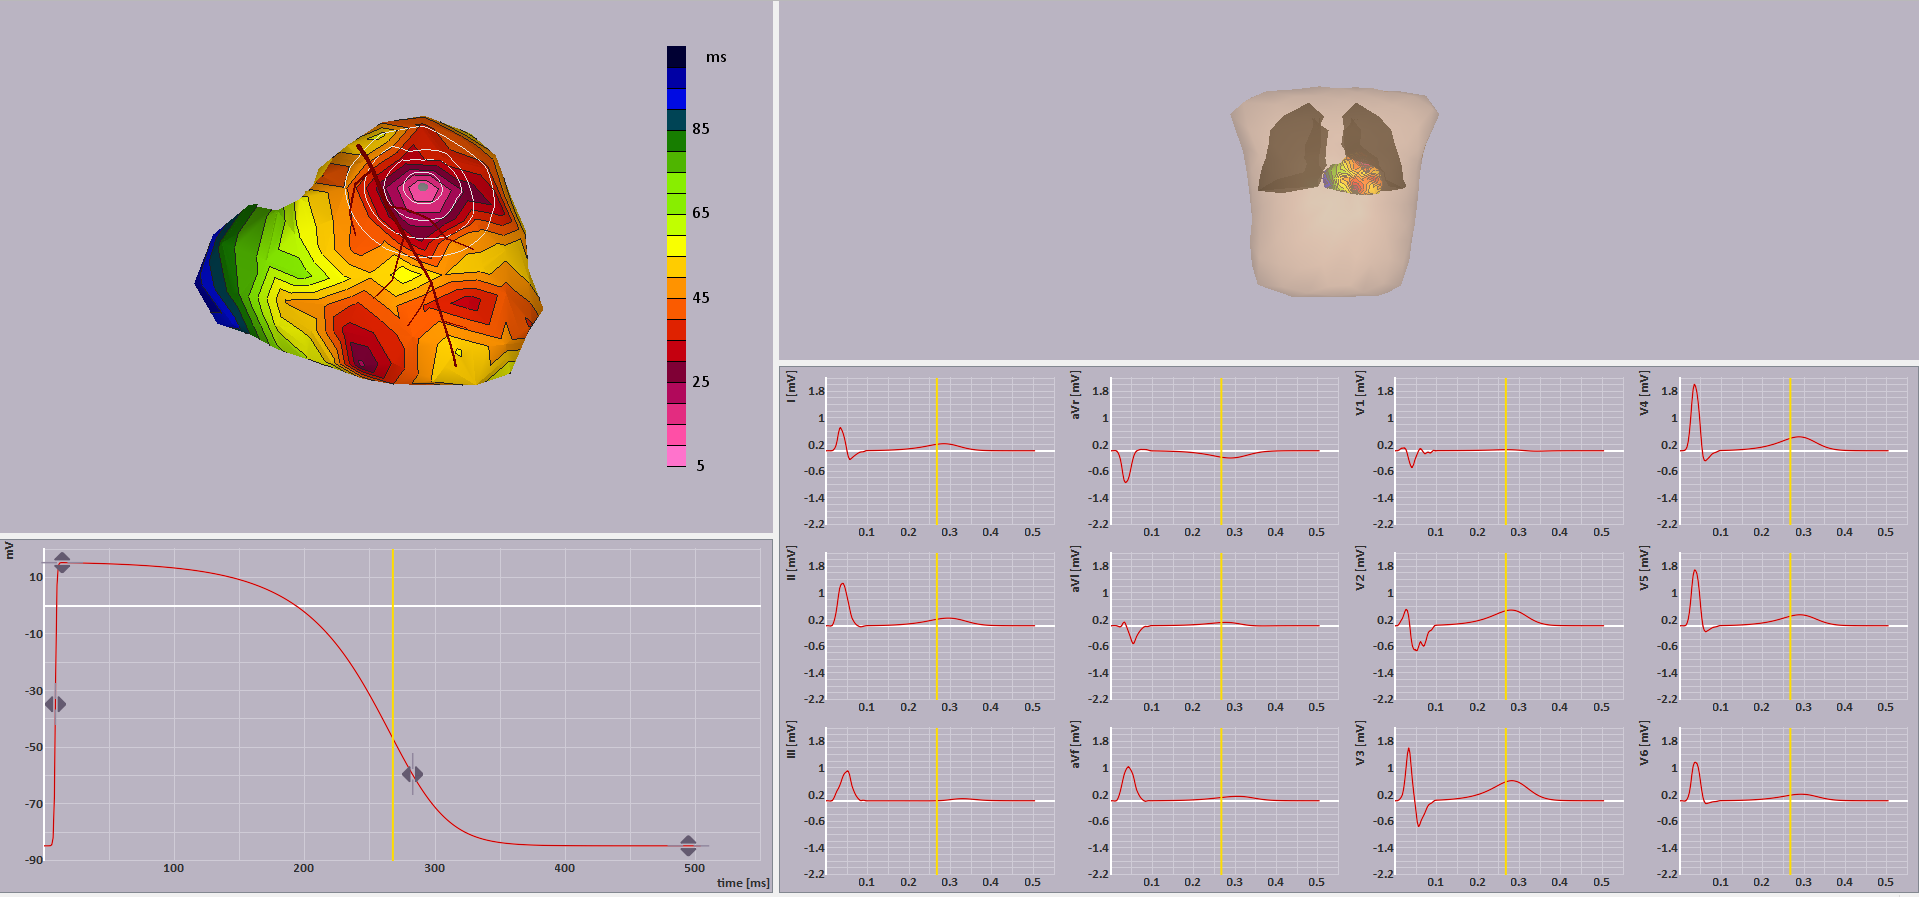
\includegraphics[width = .8\textwidth]{Figures/ActTimes.png}
	\caption{Activation map of epicardium. The area hilighted is one of early activation on the epicardium as depicted by the activation map.}
	\label{fig:ActT}
\end{figure}





